\chapter{Polut ja kierrokset}

Tämä luku käsittelee kahdenlaisia polkuja verkossa:
\begin{itemize}
\item \textit{Eulerin polku} on verkossa oleva
polku, joka kulkee tasan kerran jokaista
verkon kaarta pitkin.
\item \textit{Hamiltonin polku} on verkossa
oleva polku, joka käy tasan kerran
jokaisessa verkon solmussa.
\end{itemize}
Vaikka Eulerin ja Hamiltonin polut
näyttävät päältä päin
samantapaisilta käsitteiltä,
niihin liittyy hyvin erilaisia laskennallisia ongelmia.

Osoittautuu, että yksinkertainen verkon solmujen
asteisiin liittyvä sääntö ratkaisee, onko verkossa
Eulerin polkua, ja polun voi myös muodostaa tehokkaasti.
Sen sijaan Hamiltonin polun etsimiseen ei tunneta
mitään tehokasta algoritmia, vaan kyseessä on
NP-vaikea ongelma.

\section{Eulerin polku}

\index{Eulerin polku}

Eulerin polku (\textit{Eulerian path}) on verkossa oleva
polku, joka kulkee tarkalleen kerran jokaista kaarta pitkin.
Esimerkiksi verkossa
\begin{center}
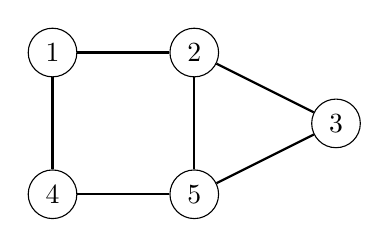
\begin{tikzpicture}[scale=0.9]
\node[draw, circle] (1) at (1,5) {$1$};
\node[draw, circle] (2) at (3,5) {$2$};
\node[draw, circle] (3) at (5,4) {$3$};
\node[draw, circle] (4) at (1,3) {$4$};
\node[draw, circle] (5) at (3,3) {$5$};

\path[draw,thick,-] (1) -- (2);
\path[draw,thick,-] (2) -- (3);
\path[draw,thick,-] (1) -- (4);
\path[draw,thick,-] (3) -- (5);
\path[draw,thick,-] (2) -- (5);
\path[draw,thick,-] (4) -- (5);
\end{tikzpicture}
\end{center}
on Eulerin polku solmusta 2 solmuun 5:
\begin{center}
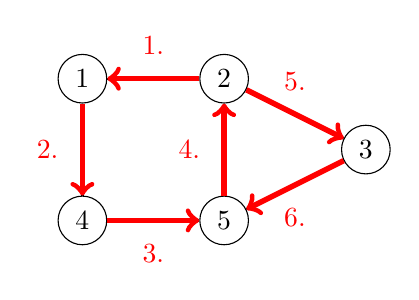
\begin{tikzpicture}[scale=0.9]
\node[draw, circle] (1) at (1,5) {$1$};
\node[draw, circle] (2) at (3,5) {$2$};
\node[draw, circle] (3) at (5,4) {$3$};
\node[draw, circle] (4) at (1,3) {$4$};
\node[draw, circle] (5) at (3,3) {$5$};

\path[draw,thick,-] (1) -- (2);
\path[draw,thick,-] (2) -- (3);
\path[draw,thick,-] (1) -- (4);
\path[draw,thick,-] (3) -- (5);
\path[draw,thick,-] (2) -- (5);
\path[draw,thick,-] (4) -- (5);

\path[draw=red,thick,->,line width=2pt] (2) -- node[font=\small,label={[red]north:1.}] {} (1);
\path[draw=red,thick,->,line width=2pt] (1) -- node[font=\small,label={[red]left:2.}] {} (4);
\path[draw=red,thick,->,line width=2pt] (4) -- node[font=\small,label={[red]south:3.}] {} (5);
\path[draw=red,thick,->,line width=2pt] (5) -- node[font=\small,label={[red]left:4.}] {} (2);
\path[draw=red,thick,->,line width=2pt] (2) -- node[font=\small,label={[red]north:5.}] {} (3);
\path[draw=red,thick,->,line width=2pt] (3) -- node[font=\small,label={[red]south:6.}] {} (5);
\end{tikzpicture}
\end{center}
\index{Eulerin kierros}
Eulerin kierros (\textit{Eulerian circuit})
on puolestaan Eulerin polku,
jonka alku- ja loppusolmu ovat samat.
Esimerkiksi verkossa
\begin{center}
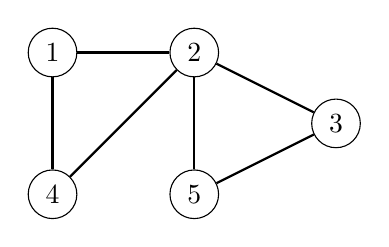
\begin{tikzpicture}[scale=0.9]
\node[draw, circle] (1) at (1,5) {$1$};
\node[draw, circle] (2) at (3,5) {$2$};
\node[draw, circle] (3) at (5,4) {$3$};
\node[draw, circle] (4) at (1,3) {$4$};
\node[draw, circle] (5) at (3,3) {$5$};

\path[draw,thick,-] (1) -- (2);
\path[draw,thick,-] (2) -- (3);
\path[draw,thick,-] (1) -- (4);
\path[draw,thick,-] (3) -- (5);
\path[draw,thick,-] (2) -- (5);
\path[draw,thick,-] (2) -- (4);
\end{tikzpicture}
\end{center}
on Eulerin kierros, jonka alku- ja loppusolmu on 1:
\begin{center}
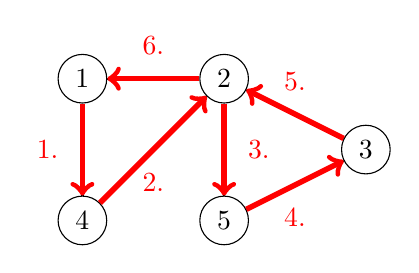
\begin{tikzpicture}[scale=0.9]
\node[draw, circle] (1) at (1,5) {$1$};
\node[draw, circle] (2) at (3,5) {$2$};
\node[draw, circle] (3) at (5,4) {$3$};
\node[draw, circle] (4) at (1,3) {$4$};
\node[draw, circle] (5) at (3,3) {$5$};

\path[draw,thick,-] (1) -- (2);
\path[draw,thick,-] (2) -- (3);
\path[draw,thick,-] (1) -- (4);
\path[draw,thick,-] (3) -- (5);
\path[draw,thick,-] (2) -- (5);
\path[draw,thick,-] (2) -- (4);

\path[draw=red,thick,->,line width=2pt] (1) -- node[font=\small,label={[red]left:1.}] {} (4);
\path[draw=red,thick,->,line width=2pt] (4) -- node[font=\small,label={[red]south:2.}] {} (2);
\path[draw=red,thick,->,line width=2pt] (2) -- node[font=\small,label={[red]right:3.}] {} (5);
\path[draw=red,thick,->,line width=2pt] (5) -- node[font=\small,label={[red]south:4.}] {} (3);
\path[draw=red,thick,->,line width=2pt] (3) -- node[font=\small,label={[red]north:5.}] {} (2);
\path[draw=red,thick,->,line width=2pt] (2) -- node[font=\small,label={[red]north:6.}] {} (1);
\end{tikzpicture}
\end{center}

\subsubsection{Olemassaolo}

Osoittautuu, että Eulerin polun ja kierroksen olemassaolo
riippuu verkon solmujen asteista.
Solmun aste on sen naapurien määrä eli niiden solmujen määrä,
jotka ovat yhteydessä solmuun kaarella.

Suuntaamattomassa verkossa on Eulerin polku,
jos kaikki kaaret ovat samassa yhtenäisessä komponentissa ja
\begin{itemize}
\item jokaisen solmun aste on parillinen \textit{tai}
\item tasan kahden solmun aste on pariton.
\end{itemize}

Ensimmäisessä tapauksessa Eulerin polku on samalla myös Eulerin kierros.
Jälkimmäisessä tapauksessa Eulerin polun alku- ja loppusolmu ovat
paritonasteiset solmut ja se ei ole Eulerin kierros.

\begin{samepage}
Esimerkiksi verkossa
\begin{center}
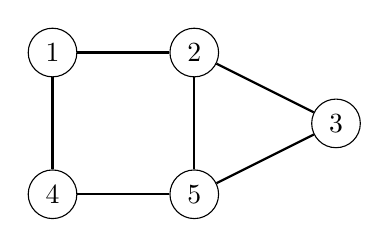
\begin{tikzpicture}[scale=0.9]
\node[draw, circle] (1) at (1,5) {$1$};
\node[draw, circle] (2) at (3,5) {$2$};
\node[draw, circle] (3) at (5,4) {$3$};
\node[draw, circle] (4) at (1,3) {$4$};
\node[draw, circle] (5) at (3,3) {$5$};

\path[draw,thick,-] (1) -- (2);
\path[draw,thick,-] (2) -- (3);
\path[draw,thick,-] (1) -- (4);
\path[draw,thick,-] (3) -- (5);
\path[draw,thick,-] (2) -- (5);
\path[draw,thick,-] (4) -- (5);
\end{tikzpicture}
\end{center}
\end{samepage}

solmujen 1, 3 ja 4 aste on 2 ja solmujen 2 ja 5 aste on 3.
Tarkalleen kahden solmun aste on pariton,
joten verkossa on Eulerin polku solmujen 2 ja 5 välillä,
mutta verkossa ei ole Eulerin kierrosta.

Jos verkko on suunnattu, tilanne on hieman hankalampi.
Silloin Eulerin polun ja kierroksen olemassaoloon
vaikuttavat solmujen lähtö- ja tuloasteet.
Solmun lähtöaste on solmusta lähtevien kaarten määrä,
ja vastaavasti solmun tuloaste on solmuun tulevien kaarten määrä.

Suunnatussa verkossa on Eulerin polku, jos
kaikki kaaret ovat samassa vahvasti yhtenäisessä
komponentissa ja
\begin{itemize}
\item jokaisen solmun lähtö- ja tuloaste on sama \textit{tai}
\item alkusolmussa lähtöaste on yhden suurempi kuin tuloaste,
loppusolmussa tuloaste on yhden suurempi kuin lähtöaste
ja kaikissa muissa solmuissa lähtö- ja tuloaste on sama.
\end{itemize}

Tilanne on vastaava kuin suuntaamattomassa verkossa:
ensimmäisessä tapauksessa Eulerin polku on myös Eulerin kierros,
ja toisessa tapauksessa verkossa on vain Eulerin polku.

Esimerkiksi verkossa
\begin{center}
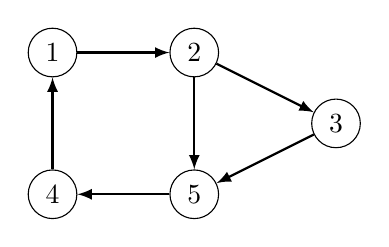
\begin{tikzpicture}[scale=0.9]
\node[draw, circle] (1) at (1,5) {$1$};
\node[draw, circle] (2) at (3,5) {$2$};
\node[draw, circle] (3) at (5,4) {$3$};
\node[draw, circle] (4) at (1,3) {$4$};
\node[draw, circle] (5) at (3,3) {$5$};

\path[draw,thick,->,>=latex] (1) -- (2);
\path[draw,thick,->,>=latex] (2) -- (3);
\path[draw,thick,->,>=latex] (4) -- (1);
\path[draw,thick,->,>=latex] (3) -- (5);
\path[draw,thick,->,>=latex] (2) -- (5);
\path[draw,thick,->,>=latex] (5) -- (4);
\end{tikzpicture}
\end{center}
solmuissa 1, 3 ja 4 sekä lähtöaste että tuloaste on 1.
Solmussa 2 tuloaste on 1 ja lähtöaste on 2,
kun taas solmussa 5 tulosate on 2 ja lähtöaste on 1.
Niinpä verkossa on Eulerin polku solmusta 2 solmuun 5:
\begin{center}
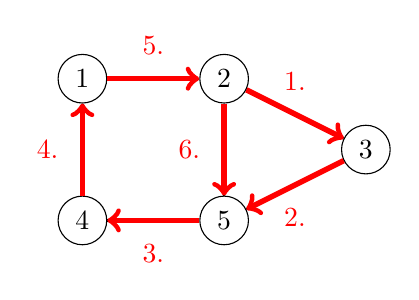
\begin{tikzpicture}[scale=0.9]
\node[draw, circle] (1) at (1,5) {$1$};
\node[draw, circle] (2) at (3,5) {$2$};
\node[draw, circle] (3) at (5,4) {$3$};
\node[draw, circle] (4) at (1,3) {$4$};
\node[draw, circle] (5) at (3,3) {$5$};

\path[draw,thick,-] (1) -- (2);
\path[draw,thick,-] (2) -- (3);
\path[draw,thick,-] (1) -- (4);
\path[draw,thick,-] (3) -- (5);
\path[draw,thick,-] (2) -- (5);
\path[draw,thick,-] (4) -- (5);

\path[draw=red,thick,->,line width=2pt] (2) -- node[font=\small,label={[red]north:1.}] {} (3);
\path[draw=red,thick,->,line width=2pt] (3) -- node[font=\small,label={[red]south:2.}] {} (5);
\path[draw=red,thick,->,line width=2pt] (5) -- node[font=\small,label={[red]south:3.}] {} (4);
\path[draw=red,thick,->,line width=2pt] (4) -- node[font=\small,label={[red]left:4.}] {} (1);
\path[draw=red,thick,->,line width=2pt] (1) -- node[font=\small,label={[red]north:5.}] {} (2);
\path[draw=red,thick,->,line width=2pt] (2) -- node[font=\small,label={[red]left:6.}] {} (5);
\end{tikzpicture}
\end{center}

\subsubsection{Muodostaminen}

Seuraavaksi esitettävä algoritmi muodostaa Eulerin kierroksen
suuntaamattomassa verkossa.
Algoritmi olettaa, että kaikki kaaret ovat samassa
komponentissa ja jokaisen solmun aste on parillinen.

Jos verkossa on kaksi paritonasteista solmua,
samalla algoritmilla voi myös muodostaa
Eulerin polun lisäämällä kaaren
paritonasteisten solmujen välille.
Tämän jälkeen verkosta voi etsiä Eulerin kierroksen,
ja lopuksi Eulerin kierroksesta saa Eulerin polun
poistamalla ylimääräisen kaaren.

Algoritmi muodostaa ensin verkkoon jonkin kierroksen,
johon kuuluu osa verkon kaarista.
Sen jälkeen algoritmi alkaa laajentaa kierrosta
lisäämällä sen osaksi uusia alikierroksia.
Tämä jatkuu niin kauan, kunnes kaikki kaaret kuuluvat
kierrokseen ja siitä on tullut Eulerin kierros.

Algoritmi laajentaa kierrosta valitsemalla jonkin
kierrokseen kuuluvan solmun $x$,
jonka kaikki kaaret eivät ole vielä mukana kierroksessa.
Algoritmi muodostaa solmusta $x$ alkaen uuden polun
kulkien vain sellaisia kaaria, jotka eivät ole
mukana kierroksessa.
Koska jokaisen solmun aste on parillinen,
ennemmin tai myöhemmin polku palaa takaisin solmuun.

\begin{samepage}
Tarkastellaan algoritmin toimintaa seuraavassa verkossa:
\begin{center}
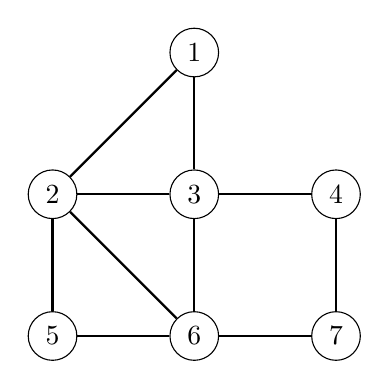
\begin{tikzpicture}[scale=0.9]
\node[draw, circle] (1) at (3,5) {$1$};
\node[draw, circle] (2) at (1,3) {$2$};
\node[draw, circle] (3) at (3,3) {$3$};
\node[draw, circle] (4) at (5,3) {$4$};
\node[draw, circle] (5) at (1,1) {$5$};
\node[draw, circle] (6) at (3,1) {$6$};
\node[draw, circle] (7) at (5,1) {$7$};

\path[draw,thick,-] (1) -- (2);
\path[draw,thick,-] (1) -- (3);
\path[draw,thick,-] (2) -- (3);
\path[draw,thick,-] (2) -- (5);
\path[draw,thick,-] (2) -- (6);
\path[draw,thick,-] (3) -- (4);
\path[draw,thick,-] (3) -- (6);
\path[draw,thick,-] (4) -- (7);
\path[draw,thick,-] (5) -- (6);
\path[draw,thick,-] (6) -- (7);
\end{tikzpicture}
\end{center}
\end{samepage}

\begin{samepage}
Oletetaan, että algoritmi aloittaa
ensimmäisen kierroksen solmusta 1.
Siitä syntyy kierros $1 \rightarrow 2 \rightarrow 3 \rightarrow 1$:
\begin{center}
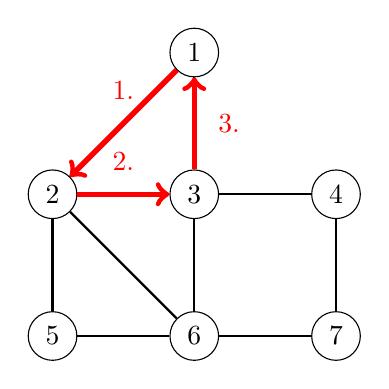
\begin{tikzpicture}[scale=0.9]
\node[draw, circle] (1) at (3,5) {$1$};
\node[draw, circle] (2) at (1,3) {$2$};
\node[draw, circle] (3) at (3,3) {$3$};
\node[draw, circle] (4) at (5,3) {$4$};
\node[draw, circle] (5) at (1,1) {$5$};
\node[draw, circle] (6) at (3,1) {$6$};
\node[draw, circle] (7) at (5,1) {$7$};

\path[draw,thick,-] (1) -- (2);
\path[draw,thick,-] (1) -- (3);
\path[draw,thick,-] (2) -- (3);
\path[draw,thick,-] (2) -- (5);
\path[draw,thick,-] (2) -- (6);
\path[draw,thick,-] (3) -- (4);
\path[draw,thick,-] (3) -- (6);
\path[draw,thick,-] (4) -- (7);
\path[draw,thick,-] (5) -- (6);
\path[draw,thick,-] (6) -- (7);

\path[draw=red,thick,->,line width=2pt] (1) -- node[font=\small,label={[red]north:1.}] {} (2);
\path[draw=red,thick,->,line width=2pt] (2) -- node[font=\small,label={[red]north:2.}] {} (3);
\path[draw=red,thick,->,line width=2pt] (3) -- node[font=\small,label={[red]east:3.}] {} (1);
\end{tikzpicture}
\end{center}
\end{samepage}

Seuraavaksi algoritmi lisää mukaan kierroksen
$2 \rightarrow 5 \rightarrow 6 \rightarrow 2$:
\begin{center}
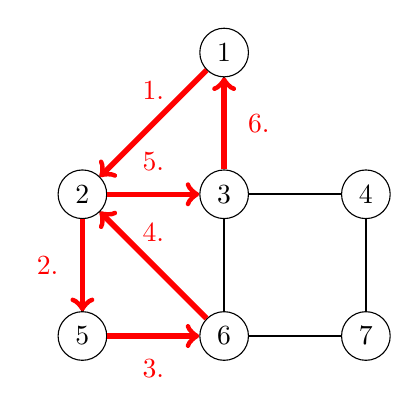
\begin{tikzpicture}[scale=0.9]
\node[draw, circle] (1) at (3,5) {$1$};
\node[draw, circle] (2) at (1,3) {$2$};
\node[draw, circle] (3) at (3,3) {$3$};
\node[draw, circle] (4) at (5,3) {$4$};
\node[draw, circle] (5) at (1,1) {$5$};
\node[draw, circle] (6) at (3,1) {$6$};
\node[draw, circle] (7) at (5,1) {$7$};

\path[draw,thick,-] (1) -- (2);
\path[draw,thick,-] (1) -- (3);
\path[draw,thick,-] (2) -- (3);
\path[draw,thick,-] (2) -- (5);
\path[draw,thick,-] (2) -- (6);
\path[draw,thick,-] (3) -- (4);
\path[draw,thick,-] (3) -- (6);
\path[draw,thick,-] (4) -- (7);
\path[draw,thick,-] (5) -- (6);
\path[draw,thick,-] (6) -- (7);

\path[draw=red,thick,->,line width=2pt] (1) -- node[font=\small,label={[red]north:1.}] {} (2);
\path[draw=red,thick,->,line width=2pt] (2) -- node[font=\small,label={[red]west:2.}] {} (5);
\path[draw=red,thick,->,line width=2pt] (5) -- node[font=\small,label={[red]south:3.}] {} (6);
\path[draw=red,thick,->,line width=2pt] (6) -- node[font=\small,label={[red]north:4.}] {} (2);
\path[draw=red,thick,->,line width=2pt] (2) -- node[font=\small,label={[red]north:5.}] {} (3);
\path[draw=red,thick,->,line width=2pt] (3) -- node[font=\small,label={[red]east:6.}] {} (1);
\end{tikzpicture}
\end{center}

Lopuksi algoritmi lisää mukaan kierroksen
$6 \rightarrow 3 \rightarrow 4 \rightarrow 7 \rightarrow 6$:
\begin{center}
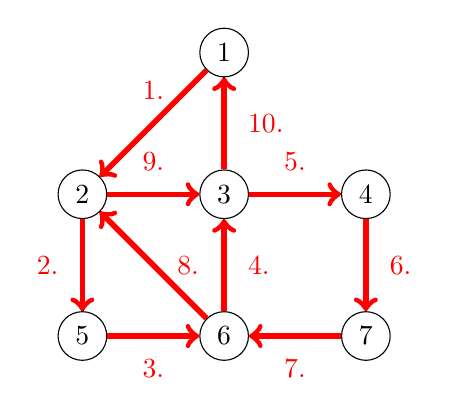
\begin{tikzpicture}[scale=0.9]
\node[draw, circle] (1) at (3,5) {$1$};
\node[draw, circle] (2) at (1,3) {$2$};
\node[draw, circle] (3) at (3,3) {$3$};
\node[draw, circle] (4) at (5,3) {$4$};
\node[draw, circle] (5) at (1,1) {$5$};
\node[draw, circle] (6) at (3,1) {$6$};
\node[draw, circle] (7) at (5,1) {$7$};

\path[draw,thick,-] (1) -- (2);
\path[draw,thick,-] (1) -- (3);
\path[draw,thick,-] (2) -- (3);
\path[draw,thick,-] (2) -- (5);
\path[draw,thick,-] (2) -- (6);
\path[draw,thick,-] (3) -- (4);
\path[draw,thick,-] (3) -- (6);
\path[draw,thick,-] (4) -- (7);
\path[draw,thick,-] (5) -- (6);
\path[draw,thick,-] (6) -- (7);

\path[draw=red,thick,->,line width=2pt] (1) -- node[font=\small,label={[red]north:1.}] {} (2);
\path[draw=red,thick,->,line width=2pt] (2) -- node[font=\small,label={[red]west:2.}] {} (5);
\path[draw=red,thick,->,line width=2pt] (5) -- node[font=\small,label={[red]south:3.}] {} (6);
\path[draw=red,thick,->,line width=2pt] (6) -- node[font=\small,label={[red]east:4.}] {} (3);
\path[draw=red,thick,->,line width=2pt] (3) -- node[font=\small,label={[red]north:5.}] {} (4);
\path[draw=red,thick,->,line width=2pt] (4) -- node[font=\small,label={[red]east:6.}] {} (7);
\path[draw=red,thick,->,line width=2pt] (7) -- node[font=\small,label={[red]south:7.}] {} (6);
\path[draw=red,thick,->,line width=2pt] (6) -- node[font=\small,label={[red]right:8.}] {} (2);
\path[draw=red,thick,->,line width=2pt] (2) -- node[font=\small,label={[red]north:9.}] {} (3);
\path[draw=red,thick,->,line width=2pt] (3) -- node[font=\small,label={[red]east:10.}] {} (1);
\end{tikzpicture}
\end{center}

Nyt kaikki kaaret ovat kierroksessa,
joten Eulerin kierros on valmis.

\subsubsection{Toteutus}

Edellä kuvattu algoritmi on mukavaa toteuttaa
niin, että solmujen vieruslistat on tallennettu joukkoina

\begin{lstlisting}
set<int> v[N];
\end{lstlisting}

jolloin verkosta on helppoa poistaa kahden solmun
välinen kaari, kun se tulee mukaan kierrokseen.

Seuraava koodi muodostaa Eulerin kierroksen
solmusta $x$ alkaen.
Se käyttää apuna pinoa
\begin{lstlisting}
stack<int> s;
\end{lstlisting}
jossa on aluksi vain kierroksen alkusolmu.
Jos pinon ylimmän solmun $u$ aste on 0,
niin algoritmi lisää solmun Eulerin kierrokseen.
Muuten algoritmi rakentaa pinon päälle uuden alikierroksen
solmusta $u$ alkaen ja poistaa kaikki alikierrokseen
kuuluvat kaaret verkosta.

\begin{lstlisting}
s.push(x);
while (!s.empty()) {
    int u = s.top(); s.pop();
    if (v[u].size() == 0) {
        // lisää solmu u Eulerin kierrokseen
    } else {
        int a = u;
        s.push(a);
        do {
            int b = *v[a].begin();
            v[a].erase(b);
            v[b].erase(a);
            s.push(b);
            a = b;
        } while (a != u);
    }
}
\end{lstlisting}
Toteutuksen aikavaativuus on $O(n+m \log n)$,
koska se käy läpi kaikki solmut ja kaaret
ja kunkin kaaren poistaminen vie aikaa $O(\log n)$.

Myös toteutus ajassa $O(n+m)$
on mahdollista mutta vaikeampaa.
Tämä vaatii verkon esittämistä niin,
että kaaria pystyy poistamaan ajassa $O(1)$,
mikä on mahdollista kahteen suuntaan
linkitettyjen vieruslistojen avulla.

\section{Hamiltonin polku}

\index{Hamiltonin polku}
Hamiltonin polku (\textit{Hamiltonian path})
on verkossa oleva polku,
joka kulkee tarkalleen kerran jokaisen solmun kautta.
Esimerkiksi verkossa
\begin{center}
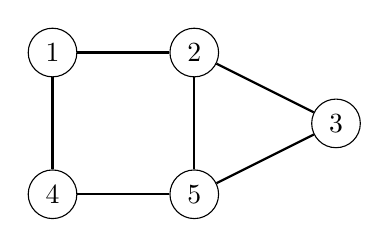
\begin{tikzpicture}[scale=0.9]
\node[draw, circle] (1) at (1,5) {$1$};
\node[draw, circle] (2) at (3,5) {$2$};
\node[draw, circle] (3) at (5,4) {$3$};
\node[draw, circle] (4) at (1,3) {$4$};
\node[draw, circle] (5) at (3,3) {$5$};

\path[draw,thick,-] (1) -- (2);
\path[draw,thick,-] (2) -- (3);
\path[draw,thick,-] (1) -- (4);
\path[draw,thick,-] (3) -- (5);
\path[draw,thick,-] (2) -- (5);
\path[draw,thick,-] (4) -- (5);
\end{tikzpicture}
\end{center}
on Hamiltonin polku solmusta 1 solmuun 3:
\begin{center}
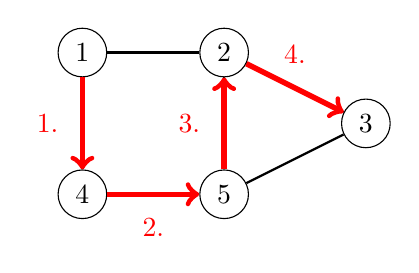
\begin{tikzpicture}[scale=0.9]
\node[draw, circle] (1) at (1,5) {$1$};
\node[draw, circle] (2) at (3,5) {$2$};
\node[draw, circle] (3) at (5,4) {$3$};
\node[draw, circle] (4) at (1,3) {$4$};
\node[draw, circle] (5) at (3,3) {$5$};

\path[draw,thick,-] (1) -- (2);
\path[draw,thick,-] (2) -- (3);
\path[draw,thick,-] (1) -- (4);
\path[draw,thick,-] (3) -- (5);
\path[draw,thick,-] (2) -- (5);
\path[draw,thick,-] (4) -- (5);

\path[draw=red,thick,->,line width=2pt] (1) -- node[font=\small,label={[red]left:1.}] {} (4);
\path[draw=red,thick,->,line width=2pt] (4) -- node[font=\small,label={[red]south:2.}] {} (5);
\path[draw=red,thick,->,line width=2pt] (5) -- node[font=\small,label={[red]left:3.}] {} (2);
\path[draw=red,thick,->,line width=2pt] (2) -- node[font=\small,label={[red]north:4.}] {} (3);
\end{tikzpicture}
\end{center}

\index{Hamiltonin kierros}
Jos Hamiltonin polun alku- ja loppusolmu on sama,
kyseessä on Hamiltonin kierros (\textit{Hamiltonian circuit}).
Äskeisessä verkossa on myös
Hamiltonin kierros, jonka alku- ja loppusolmu on solmu 1:
\begin{center}
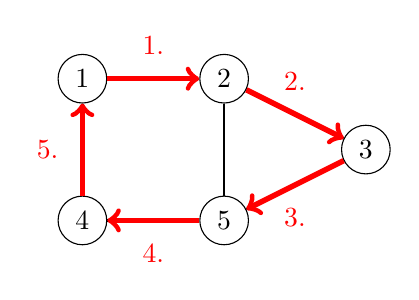
\begin{tikzpicture}[scale=0.9]
\node[draw, circle] (1) at (1,5) {$1$};
\node[draw, circle] (2) at (3,5) {$2$};
\node[draw, circle] (3) at (5,4) {$3$};
\node[draw, circle] (4) at (1,3) {$4$};
\node[draw, circle] (5) at (3,3) {$5$};

\path[draw,thick,-] (1) -- (2);
\path[draw,thick,-] (2) -- (3);
\path[draw,thick,-] (1) -- (4);
\path[draw,thick,-] (3) -- (5);
\path[draw,thick,-] (2) -- (5);
\path[draw,thick,-] (4) -- (5);

\path[draw=red,thick,->,line width=2pt] (1) -- node[font=\small,label={[red]north:1.}] {} (2);
\path[draw=red,thick,->,line width=2pt] (2) -- node[font=\small,label={[red]north:2.}] {} (3);
\path[draw=red,thick,->,line width=2pt] (3) -- node[font=\small,label={[red]south:3.}] {} (5);
\path[draw=red,thick,->,line width=2pt] (5) -- node[font=\small,label={[red]south:4.}] {} (4);
\path[draw=red,thick,->,line width=2pt] (4) -- node[font=\small,label={[red]left:5.}] {} (1);
\end{tikzpicture}
\end{center}

\subsubsection{Olemassaolo}

Hamiltonin polun olemassaoloon ei tiedetä
mitään verkon rakenteeseen liittyvää ehtoa,
jonka voisi tarkistaa tehokkaasti.
Joissakin erikoistapauksissa voidaan silti sanoa
varmasti, että verkossa on Hamiltonin polku.

Yksinkertainen havainto on, että jos verkko on täydellinen
eli jokaisen solmun välillä on kaari,
niin siinä on Hamiltonin polku.
Myös vahvempia tuloksia on saatu aikaan:

\begin{itemize}
\item
\index{Diracin lause}
\textit{Diracin lause}:
Jos jokaisen verkon solmun aste on $n/2$ tai suurempi,
niin verkossa on Hamiltonin polku.
\item
\index{Oren lause}
\textit{Oren lause}:
Jos jokaisen ei-vierekkäisen solmuparin asteiden summa
on $n$ tai suurempi,
niin verkossa on Hamiltonin polku.
\end{itemize}

Yhteistä näissä ja muissa tuloksissa on,
että ne takaavat Hamiltonin polun olemassaolon,
jos verkossa on \textit{paljon} kaaria.
Tämä on ymmärrettävää, koska mitä enemmän
kaaria verkossa on, sitä enemmän mahdollisuuksia
Hamiltonin polun muodostamiseen on olemassa.

\subsubsection{Muodostaminen}

Koska Hamiltonin polun olemassaoloa ei voi tarkastaa tehokkaasti,
on selvää, että polkua ei voi myöskään muodostaa tehokkaasti,
koska muuten polun olemassaolon voisi selvittää yrittämällä
muodostaa sen.

Yksinkertaisin tapa etsiä Hamiltonin polkua on käyttää
peruuttavaa hakua, joka käy läpi kaikki vaihtoehdot
polun muodostamiseen.
Tällaisen algoritmin aikavaativuus on ainakin luokkaa $O(n!)$,
koska $n$ solmusta voidaan muodostaa $n!$ järjestystä,
jossa ne voivat esiintyä polulla.

Tehokkaampi tapa perustuu dynaamiseen ohjelmointiin
luvun 10.4 tapaan.
Ideana on määritellä funktio $f(s,x)$,
jossa $s$ on verkon solmujen osajoukko ja
$x$ on yksi osajoukon solmuista.
Funktio kertoo, onko olemassa Hamiltonin polkua,
joka käy läpi joukon $s$ solmut päätyen solmuun $x$.
Tällainen ratkaisu on mahdollista toteuttaa ajassa $O(2^n n^2)$.

\section{De Bruijnin jono}

\index{de Bruijnin jono}

De Bruijnin jono (\textit{de Bruijn sequence})
on lyhin $k$-merkkisen aakkoston merkkijono,
jonka osajonoina ovat kaikki mahdolliset
$n$ merkin yhdistelmät.
Esimerkiksi kun $k=2$ ja $n=3$,
niin eräs de Bruijnin jono on

\[0001011100.\]

Tämän merkkijonon osajonoina ovat kaikki 3 merkin yhdistelmät
000, 001, 010, 011, 100, 101, 110 ja 111.

Osoittautuu, että lyhimmän merkkijonon
pituus on aina $k^n+n-1$, jolloin jokainen
$n$ merkin osajono esiintyy tarkalleen
kerran merkkijonossa.
Tällainen merkkijono
vastaa Eulerin kierrosta sopivasti
muodostetussa verkossa.

Ideana on muodostaa verkko niin,
että jokaisessa solmussa on $n-1$
merkin yhdistelmä ja liikkuminen
kaarta pitkin muodostaa uuden
$n$ merkin yhdistelmän.
Esimerkin tapauksessa verkosta tulee seuraava:

\begin{center}
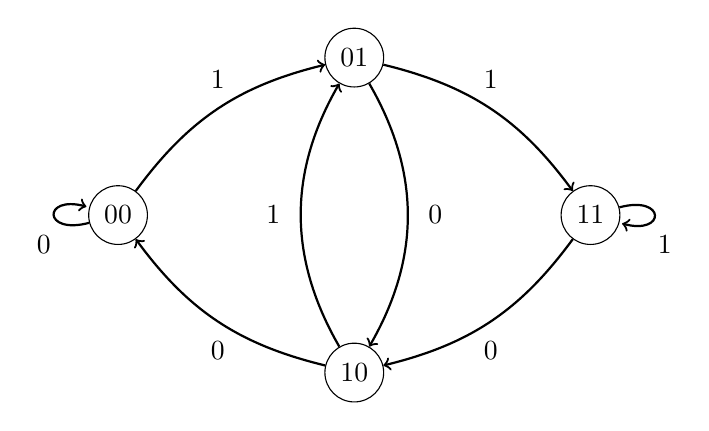
\begin{tikzpicture}
\node[draw, circle] (00) at (-3,0) {00};
\node[draw, circle] (11) at (3,0) {11};
\node[draw, circle] (01) at (0,2) {01};
\node[draw, circle] (10) at (0,-2) {10};

\path[draw,thick,->] (00) edge [bend left=20] node[font=\small,label=1] {} (01);
\path[draw,thick,->] (01) edge [bend left=20] node[font=\small,label=1] {} (11);
\path[draw,thick,->] (11) edge [bend left=20] node[font=\small,label=below:0] {} (10);
\path[draw,thick,->] (10) edge [bend left=20] node[font=\small,label=below:0] {} (00);

\path[draw,thick,->] (01) edge [bend left=30] node[font=\small,label=right:0] {} (10);
\path[draw,thick,->] (10) edge [bend left=30] node[font=\small,label=left:1] {} (01);

\path[draw,thick,-] (00) edge [loop left] node[font=\small,label=below:0] {} (00);
\path[draw,thick,-] (11) edge [loop right] node[font=\small,label=below:1] {} (11);
\end{tikzpicture}
\end{center}

Eulerin kierros tässä verkossa tuottaa merkkijonon,
joka sisältää kaikki $n$ merkin yhdistelmät,
kun mukaan otetaan aloitussolmun merkit sekä
kussakin kaaressa olevat merkit.
Aloitussolmussa on $n-1$ merkkiä ja kaarissa
on $k^n$ merkkiä, joten tuloksena on
lyhin mahdollinen merkkijono.

\section{Ratsun kierros}

\index{ratsun kierros}

Ratsun kierros (\textit{knight's tour}) on tapa liikuttaa ratsua
shakin sääntöjen mukaisesti $n \times n$ -kokoisella
shakkilaudalla niin,
että ratsu käy tarkalleen kerran jokaisessa ruudussa.
Kierros on \textit{suljettu}, jos ratsu palaa lopuksi alkuruutuun,
ja muussa tapauksessa se on \textit{avoin}.

Esimerkiksi tapauksessa $5 \times 5$ yksi ratsun kierros on seuraava:

\begin{center}
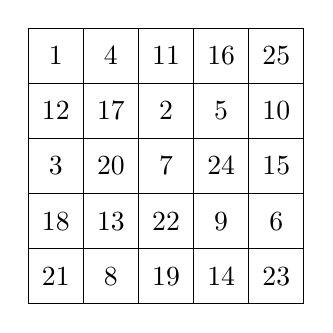
\begin{tikzpicture}[scale=0.7]
\draw (0,0) grid (5,5);
\node at (0.5,4.5) {$1$};
\node at (1.5,4.5) {$4$};
\node at (2.5,4.5) {$11$};
\node at (3.5,4.5) {$16$};
\node at (4.5,4.5) {$25$};
\node at (0.5,3.5) {$12$};
\node at (1.5,3.5) {$17$};
\node at (2.5,3.5) {$2$};
\node at (3.5,3.5) {$5$};
\node at (4.5,3.5) {$10$};
\node at (0.5,2.5) {$3$};
\node at (1.5,2.5) {$20$};
\node at (2.5,2.5) {$7$};
\node at (3.5,2.5) {$24$};
\node at (4.5,2.5) {$15$};
\node at (0.5,1.5) {$18$};
\node at (1.5,1.5) {$13$};
\node at (2.5,1.5) {$22$};
\node at (3.5,1.5) {$9$};
\node at (4.5,1.5) {$6$};
\node at (0.5,0.5) {$21$};
\node at (1.5,0.5) {$8$};
\node at (2.5,0.5) {$19$};
\node at (3.5,0.5) {$14$};
\node at (4.5,0.5) {$23$};
\end{tikzpicture}
\end{center}

Ratsun kierros shakkilaudalla vastaa Hamiltonin polkua verkossa,
jonka solmut ovat ruutuja ja kahden solmun välillä on kaari,
jos ratsu pystyy siirtymään solmusta toiseen shakin sääntöjen mukaisesti.

Peruuttava haku on luonteva menetelmä ratsun kierroksen muodostamiseen.
Hakua voi tehostaa erilaisilla heuristiikoilla,
jotka pyrkivät ohjaamaan ratsua niin, että kokonainen kierros
tulee valmiiksi nopeasti.

\subsubsection{Warnsdorffin sääntö}

\index{heuristiikka}
\index{Warnsdorffin sääntö}

Warnsdorffin sääntö on yksinkertainen mutta käytännössä hyvä heuristiikka
ratsun kierroksen etsimiseen.
Sen avulla on mahdollista löytää nopeasti ratsun kierros
suurestakin ruudukosta.

Heuristiikassa on ideana siirtää ratsua aina niin,
että se päätyy ruutuun, josta on mahdollisimman vähän
mahdollisuuksia jatkaa kierrosta.
Esimerkiksi seuraavassa tilanteessa on valittavana
viisi ruutua, joihin ratsu voi siirtyä:
\begin{center}
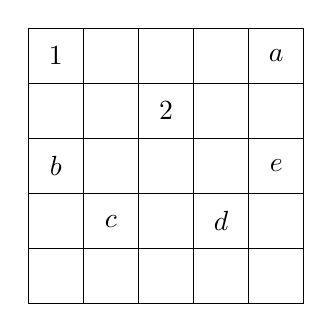
\begin{tikzpicture}[scale=0.7]
\draw (0,0) grid (5,5);
\node at (0.5,4.5) {$1$};
\node at (2.5,3.5) {$2$};
\node at (4.5,4.5) {$a$};
\node at (0.5,2.5) {$b$};
\node at (4.5,2.5) {$e$};
\node at (1.5,1.5) {$c$};
\node at (3.5,1.5) {$d$};
\end{tikzpicture}
\end{center}
Tässä tapauksessa Warnsdorffin sääntö valitsee ruudun $a$,
koska tämän valinnan jälkeen on vain yksi mahdollisuus
jatkaa kierrosta. Muissa valinnoissa mahdollisuuksia olisi kolme.
